\documentclass[xcolor=pdflatex,dvipsnames,table]{beamer}
\usepackage{epsfig,graphicx}
\usepackage{palatino}
\usepackage{fancybox}
\usepackage{relsize}
\usepackage[procnames]{listings}
\usepackage{hyperref}
\usepackage{qtree} % needed?
\usepackage{booktabs}
\usepackage{dirtree}
\usepackage[normalem]{ulem}


% fatter TT font
\renewcommand*\ttdefault{txtt}
% another TT, suggested by Alex
% \usepackage{inconsolata}
% \usepackage[T1]{fontenc} % needed as well?


\newcommand{\scale}{0.7}

\newcommand{\todo}[1]{{\emph{TODO: #1}}}
\newcommand{\martin}[1]{{\color{blue} Martin: #1}}
\newcommand{\abcdef}[1]{{\color{red} Author2: #1}}

% uncomment following for final submission
%\renewcommand{\todo}[1]{}
%\renewcommand{\martin}[1]{}
%\renewcommand{\author2}[1]{}

\newcommand{\code}[1]{{\texttt{#1}}}

\hypersetup{
  linkcolor  = black,
%  citecolor  = blue,
  urlcolor   = blue,
  colorlinks = true,
}

\beamertemplatenavigationsymbolsempty
\setbeamertemplate{footline}[frame number]





\newif\ifbook
% shared in slides and book

\lstdefinelanguage{chisel}{
  morekeywords={abstract,case,catch,class,def,%
    do,else,extends,false,final,finally,%
    for,if,implicit,import,match,mixin,%
    new,null,object,override,package,%
    private,protected,requires,return,sealed,%
    super,this,throw,trait,true,try,%
    type,val,var,while,with,yield},
  otherkeywords={=>,<-,<\%,<:,>:,\#,@},
  sensitive=true,
  morecomment=[l]{//},
  morecomment=[n]{/*}{*/},
  morestring=[b]",
  morestring=[b]',
  morestring=[b]"""
}

\usepackage{color}
\definecolor{dkgreen}{rgb}{0,0.6,0}
\definecolor{gray}{rgb}{0.5,0.5,0.5}
\definecolor{mauve}{rgb}{0.58,0,0.82}

% Default settings for code listings
\ifbook
\lstset{%frame=lines,
  language=chisel,
  aboveskip=3mm,
  belowskip=3mm,
  showstringspaces=false,
  columns=fixed, % basewidth=\mybasewidth,
  basicstyle={\small\ttfamily},
  numbers=none,
  numberstyle=\footnotesize,
  % identifierstyle=\color{red},
  breaklines=true,
  breakatwhitespace=true,
  procnamekeys={def, val, var, class, trait, object, extends},
  % procnamestyle=\ttfamily,
  tabsize=2,
  float
}
\else
\lstset{%frame=lines,
  language=chisel,
  aboveskip=3mm,
  belowskip=3mm,
  showstringspaces=false,
  columns=fixed, % basewidth=\mybasewidth,
  basicstyle={\small\ttfamily},
  numbers=none,
  numberstyle=\footnotesize\color{gray},
  % identifierstyle=\color{red},
  keywordstyle=\color{blue},
  commentstyle=\color{dkgreen},
  stringstyle=\color{mauve},
  breaklines=true,
  breakatwhitespace=true,
  procnamekeys={def, val, var, class, trait, object, extends},
  procnamestyle=\ttfamily\color{red},
  tabsize=2,
  float
}
\fi

\lstnewenvironment{chisel}[1][]
{\lstset{language=chisel,#1}}
{}

\newcommand{\shortlist}[1]{{\lstinputlisting[nolol]{#1}}}

\newcommand{\longlist}[3]{{\lstinputlisting[float, caption={#2}, label={#3}, frame=tb, captionpos=b]{#1}}}

\newcommand{\verylonglist}[3]{{\lstinputlisting[caption={#2}, label={#3}, frame=tb, captionpos=b]{#1}}}


\title{Unused Stuff}
\author{Martin Schoeberl}
\date{\today}
\institute{Technical University of Denmark\\
Embedded Systems Engineering}

\begin{document}

\begin{frame}
\titlepage
\end{frame}


\begin{frame}[fragile]{TODO}
\begin{itemize}
\item xxx
\end{itemize}
\end{frame}


\begin{frame}[fragile]{Chisel VHDL Comparison}
\begin{columns}
\column{0.5\textwidth}
\begin{chisel}
class DecodeExecute extends Bundle {
  val rs1 = UInt(32.W)
  val rs2 = UInt(32.W)
  val immVal = UInt(32.W)
  val aluOp = new AluOp()
}
\end{chisel}
\column{0.5\textwidth}
\begin{verbatim}
VHDL code here
\end{verbatim}
\end{columns}
Also show latch and and using a button as clock
\end{frame}

\begin{frame}[fragile]{Below Stuff Moved Over}
\begin{itemize}
\item From tutorial
\item Maybe used in the future
\end{itemize}
\end{frame}



\begin{frame}[fragile]{Component Generation}
\begin{chisel}
val cores = new Array[Module](32)

for (j <- 0 until 32)
  cores(j) = Module(new CPU())
\end{chisel}
\begin{itemize}
\item Use Scala array to collect components
\item Generation with a Scala loop
\end{itemize}
\end{frame}

\begin{frame}[fragile]{Conditional Component Generation}
\begin{chisel}
val icache =
  if (TYPE == METHOD)
    Module(new MCache())
  else if (TYPE == LINE)
    Module(new ICache())
  else
    ChiselError.error("Unsupported Type")
\end{chisel}
\begin{itemize}
\item Use Scala if/else for conditional component types
\item Code example from Patmos
\item We parse an XML file for the configuration
\end{itemize}
\end{frame}

\begin{frame}[fragile]{Logic Generation}
\begin{itemize}
\item Read a file into a table
\begin{itemize}
\item E.g., to read in ROM content for a processor
\end{itemize}
\item Generate a truth table algorithmically
\begin{itemize}
\item E.g., generate binary to BCD translation
\end{itemize}
\item Use the full power of Scala
\end{itemize}
\begin{chisel}
val byteArray = Files.readAllBytes(Paths.get(fileName))
val arr = new Array[Bits](byteArray.length)
for (i <- 0 until byteArray.length) {
  arr(i) = Bits(byteArray(i), 8)
}
val rom = Vec[Bits](arr)
\end{chisel}
\end{frame}
%%%%%%%%%%%%%%%%%
%\begin{frame}[fragile]{zzz}
%\begin{chisel}
%code
%\end{chisel}
%\begin{itemize}
%\item xxx
%\item xxx
%\item xxx
%\end{itemize}
%\end{frame}
%
%\begin{frame}[fragile]{yyy}
%\begin{itemize}
%\item xxx
%\item xxx
%\item xxx
%\item xxx
%\item xxx
%\end{itemize}
%\end{frame}
%%%%%%%%%%%%%%%%%


%\begin{frame}[fragile]{Chisel has a Multiplexer}
\begin{figure}
  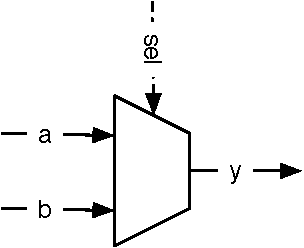
\includegraphics[scale=\scale]{../figures/mux}
\end{figure}
\shortlist{../code/mux.txt}
\begin{itemize}
\item So what?
\item Wait... What type is \code{a} and \code{b}?
\begin{itemize}
\item Can be any Chisel type!
\end{itemize}
\end{itemize}
\end{frame}

\begin{frame}[fragile]{Chisel has a Generic Multiplexer}
\begin{figure}
  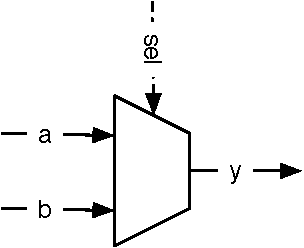
\includegraphics[scale=\scale]{../figures/mux}
\end{figure}
\shortlist{../code/mux.txt}
\begin{itemize}
\item SW people may not be impressed
\item They have generics since Java 1.5 in 2004
\begin{itemize}
\item \code{List<Flowers> != List<Cars>}
\end{itemize}
\end{itemize}
\end{frame}


\begin{frame}[fragile]{Generics in Hardware Construction}
\begin{itemize}
\item Chisel supports generic classes with type parameters
\item Write hardware generators independent of concrete type
\item This is a multiplexer \emph{generator}
\end{itemize}
\shortlist{../code/param_func.txt}
\end{frame}

\begin{frame}[fragile]{Put Generics Into Use}
\begin{itemize}
\item Let us implement a generic FIFO
\item Use the generic ready/valid interface from Chisel
\end{itemize}
\shortlist{../code/fifo_decoupled.txt}
\end{frame}

\begin{frame}[fragile]{Define the FIFO Interface}
\shortlist{../code/fifo_io.txt}
\begin{itemize}
\item We need enqueueing and dequeueing ports
\item Note the \code{Flipped}
\begin{itemize}
\item It switches the direction of ports
\item No more double definitions of an interface
\end{itemize}
\end{itemize}
\end{frame}

\begin{frame}[fragile]{But What FIFO Implementation?}
\begin{itemize}
\item Bubble FIFO (good for low data rate)
\item Double buffer FIFO (fast restart)
\item FIFO with memory and pointers (for larger buffers)
\begin{itemize}
\item Using flip-flops
\item Using on-chip memory
\end{itemize}
\item And some more...
\end{itemize}
\begin{itemize}
\item This calls for object-oriented \sout{programming} \emph{hardware construction}
\end{itemize}
\end{frame}

\begin{frame}[fragile]{Abstract Base Class and Concrete Extension}
\shortlist{../code/fifo_abstract.txt}
\begin{itemize}
\item May contain common code
\item Extend by concrete classes
\end{itemize}
\begin{chisel}
class BubbleFifo[T <: Data](gen: T, depth: Int) extends Fifo(gen: T, depth: Int) {
\end{chisel}
\end{frame}



\begin{frame}[fragile]{Select a Concrete FIFO Implementation}
\begin{itemize}
\item Decide at hardware generation
\item Can use all Scala/Java power for the decision
\begin{itemize}
\item Connect to a web service, get \sout{Google} Alphabet stock price, and decide on which to use ;-)
\item For sure a silly idea, but you see what is possible...
\item Developers may find clever use of the Scala/Java power
\item We could present a GUI to the user to select from
\end{itemize}
\item We use XML files parsed at hardware generation time
\item End of TCL, Python,... generated hardware
\end{itemize}
\end{frame}

\begin{frame}[fragile]{Binary to BCD Conversion for VHDL}
\begin{figure}
    \centering
    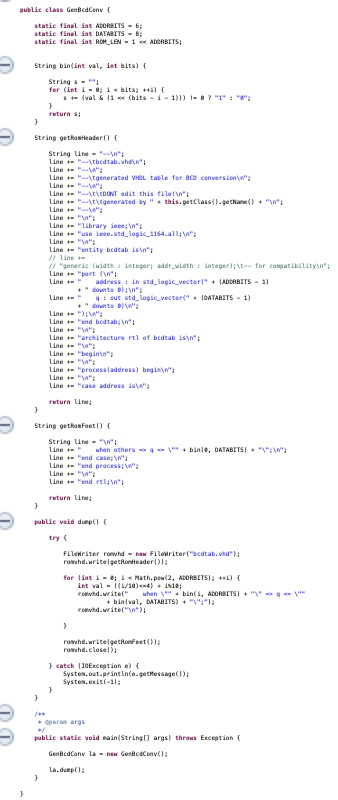
\includegraphics[scale=0.6]{JavaBCD}
\end{figure}
\end{frame}

\begin{frame}[fragile]{Java Program}
\begin{itemize}
\item Generates a VHDL table
\item The core code is:
\end{itemize}
\begin{chisel}
for (int i = 0; i < Math.pow(2, ADDRBITS); ++i) {
    int val = ((i/10)<<4) + i%10;
    // write out VHDL code for each line
\end{chisel}
\begin{itemize}
\item With all boilerplate 118 LoC
\end{itemize}
\end{frame}

\begin{frame}[fragile]{Chisel Version of Binary to BCD Conversion}
%\begin{chisel}
%  val array = new Array[Int](256)
%  for (i <- 0 to 99) {
%    array(i) = ((i/10)<<4) + i%10
%  }
%  val table = VecInit(array.map(_.U(8.W)))
%\end{chisel}
\begin{chisel}
  val table = Wire(Vec(100, UInt(8.W)))
  for (i <- 0 until 100) {
    table(i) := (((i/10)<<4) + i%10).U
  }
  val bcd = table(bin)
\end{chisel}
\begin{itemize}
\item Directly generates the hardware table as a \code{Vec}
\item At hardware construction time
\item In the same language
\end{itemize}
\end{frame}

\begin{frame}[fragile]{Use Functional Programming for Generators}
\shortlist{../code/fun_first.txt}
\shortlist{../code/fun_func_lit.txt}
\shortlist{../code/fun_reduce_tree.txt}
\begin{itemize}
\item This is a simple example
\item What about an arbiter tree with fair arbitration?
\end{itemize}
\end{frame}

%\begin{frame}[fragile]{XXX}
%\begin{itemize}
%\item TODO: s4noc connection is part of the generator story
%\item
%\item
%\end{itemize}
%\end{frame}
%
%\begin{frame}[fragile]{XXX}
%\begin{itemize}
%\item
%\item
%\item
%\end{itemize}
%\end{frame}



\begin{frame}[fragile]{Generation Slides (include) are missing here}
\begin{itemize}
\item 
\end{itemize}
\end{frame}

\begin{frame}[fragile]{Combinational (Truth) Table Generation}
\begin{chisel}
val arr = new Array[Bits](length)
for (i <- 0 until length) {
  arr(i) = ...
}
val rom = Vec[Bits](arr)
\end{chisel}
\begin{itemize}
\item Generate a table in a Scala array
\item Use that array as input for a Chisel \code{Vec}
\item Generates a logic table at hardware construction time
\end{itemize}
\end{frame}

\begin{frame}[fragile]{BCD Generation Example}
\begin{itemize}
\item Explain BCD with examples
\item Show code
\end{itemize}
\end{frame}

\begin{frame}[fragile]{Ideas for Runtime Table Generation}
\begin{itemize}
\item Assembler in Scala/Java generates the boot ROM
\item Table with a \code{sin} function
\item Binary to BCD conversion
\item Schedule table for a TDM based network-on-chip
\item 
\item More ideas?
\end{itemize}
\end{frame}

\begin{frame}[fragile]{Memory}
\begin{chisel}
val mem = Mem(Bits(width = 8), size)

// write
when(wrEna) {
  mem(wrAddr) := wrData
}

// read
val rdAddrReg = Reg(next = rdAddr)
rdData := mem(rdAddrReg)
\end{chisel}
\begin{itemize}
\item TODO: this is the old memory
\item Write is synchronous
\item Read can be asynchronous or synchronous
\item But there are no asynchronous memories in an FPGA
\end{itemize}
\end{frame}

\begin{frame}[fragile]{Factory Methods}
\begin{itemize}
\item Simpler component creation and use
\item Usage similar to built in components, such as \code{Mux}
\end{itemize}
\begin{chisel}
val myAdder = Adder(x, y)
\end{chisel}
\begin{itemize}
\item A little bit more work on component side
\item Define an \code{apply} method on the companion object that returns the component
\end{itemize}
\begin{chisel}
object Adder {
  def apply(a: UInt, b: UInt) = {
    val adder = Module(new Adder)
    adder.io.a := a
    adder.io.b := b
    adder.io.result
  }
}
\end{chisel}
\end{frame}


\begin{frame}[fragile]{Generic Components}
\begin{chisel}
val c = Mux(cond, a, b)
\end{chisel}
\begin{itemize}
\item This is a multiplexer
\item Input can be any type
\end{itemize}
\end{frame}




\begin{frame}[fragile]{A Tiny ALU: IO Connection}
\begin{chisel}
class Alu extends Module {
  val io = IO(new Bundle {
    val fn = Input(UInt(2.W))
    val a = Input(UInt(4.W))
    val b = Input(UInt(4.W))
    val result = Output(UInt(4.W))
  })

  // Use shorter variable names
  val fn = io.fn
  val a = io.a
  val b = io.b
\end{chisel}
\end{frame}

\begin{frame}[fragile]{A Tiny ALU: The Function}
\begin{chisel}
  val result = Wire(UInt(4.W))
  // some default value is needed
  result := 0.U

  // The ALU selection
  switch(fn) {
    is(0.U) { result := a + b }
    is(1.U) { result := a - b }
    is(2.U) { result := a | b }
    is(3.U) { result := a & b }
  }

  // Output on the LEDs
  io.result := result
}
\end{chisel}
\end{frame}

\begin{frame}[fragile]{Testing the ALU}
\begin{itemize}
\item Compute the expected result in Scala
\end{itemize}
\begin{chisel}
  // This is exhaustive testing,
  // which usually is impossible
  for (a <- 0 to 15) {
    for (b <- 0 to 15) {
      for (op <- 0 to 3) {
        val result =
          op match {
            case 0 => a + b
            case 1 => a - b
            case 2 => a | b
            case 3 => a & b
          }
        val resMask = result & 0x0f
\end{chisel}

\end{frame}

\begin{frame}[fragile]{Testing the ALU}
\begin{itemize}
\item Compare the Scala computed result with the hardware result
\end{itemize}
\begin{chisel}
        poke(dut.io.fn, op)
        poke(dut.io.a, a)
        poke(dut.io.b, b)
        step(1)
        expect(dut.io.result, resMask)
      }
    }
  }
\end{chisel}
\end{frame}


\begin{frame}[fragile]{Summary}
\begin{itemize}
\item Chisel is a small language
\item Embedding it in Scala gives the power
\item We can write circuit generators
\item We can to co-simulation
\item We just scratched the surface
\end{itemize}
\end{frame}


\end{document}

%\begin{frame}[fragile]{xxx}
%\begin{itemize}
%\item yyy
%\end{itemize}
%\end{frame}
